\chapter{Stand van zaken}
\label{ch:stand-van-zaken}

Bij dit hoofdstuk wordt de literatuurstudie besproken. Qua literatuur is er gezocht naar info die te maken heeft met de 3 grote pijlers van dit onderzoek. Eerst wordt besproken wat de literatuur vermeldt over studenten aan een hogeschool en hun gedrag. Vervolgens bekijkt men wat de devices zijn die studenten meebrengen naar school en welk effect ze mogelijks kunnen hebben. Als laatste wordt gekeken naar de resultaten die studenten behalen en de mogelijke oorzaken/gevolgen.

\textcite{Johnson2017} onderzochten hoe academisch de smartphone werd gebruikt bij studenten van een business-school. Hoewel hun onderzoek niet statistisch volledig significant was, konden zij toch concluderen dat smartphones een impact hadden op de studenten, soms positief, soms negatief. Positief was bijvoorbeeld de mogelijkheid om voor elk probleem dat de student tegenkwam bij schooltaken een applicatie te downloaden op hun smartphone die het probleem deels voor hun kon oplossen. Ook heeft de komst van de laptops ervoor gezorgd dat studenten hun taken zorgvuldiger en beter op tijd kunnen afronden. Zij merkten ook in hun onderzoek dat het bezit van een smartphone of ander elektronisch device een boost gaf aan hun ego of imago in de klas. Negatief voor de studenten was dat de apparaten voor afleiding zorgen en als gevolg daarvan de punten lager zijn. \textcite{Hossain2016} hun onderzoek sluit hierbij aan. Zij vonden dat onder 316 studenten ongeveer 2/3 van de studenten hun smartphone gebruikten om academische informatie op te zoeken. 

Deze bovenstaande onderzoeken duiden aan dat studenten wel degelijk hun devices voor schooldoeleinden gebruiken en dit ook zelf duidelijk aangeven. Ze kunnen gemakkelijker samenvattingen schrijven, sneller een vraag stellen aan medestudenten… Toch blijft de vraag hoeveel tijd er werkelijk besteed wordt aan deze schooltaken, en hoeveel tijd er gaat naar ontspanning op de smartphone. Hier wil het onderzoek in een later stadium een beter antwoord op geven.

\textcite{Alfawareh2014} keken naar het aantal studenten van een universiteit in Saudi-Arabië dat een smartphone meenam naar school. Zij vonden dat wel 94,4 procent van de ondervraagden in het bezit was van een smartphone. Het is dus ook te verwachten in de resultaten van dit onderzoek dat meer dan 95 procent van de ondervraagden een of ander elektronisch apparaat altijd meenemen naar de les. Iets meer dan 90 procent van de ondervraagden gebruikten hun smartphone om in te loggen op het portaal van de universiteit. Opvallendste voor dit onderzoek is dat uit hun resultaten bleek dat maar 54,49 procent van de ondervraagde personen hun smartphone altijd of soms gebruikte om klasmateriaal (slides, pdf’s, nota’s) te downloaden of te gebruiken voor een les. Gebruik van laptops werd hier niet onderzocht. Het Student Mobile Device Survey \autocite{Harris2015} heeft wel gekeken naar het gebruik van laptops. Zij vonden in hun onlineonderzoek in de Verenigde Staten dat verspreid werd onder 1211 hogeschoolstudenten tussen de 18-30 jaar dat 87 procent van de hogeschoolstudenten hun laptop elke week gebruiken voor schoolwerk, terwijl maar 64 procent gebruik maakt van hun smartphone hiervoor en maar 40 procent een tablet gebruikt. Hieruit blijkt dus dat smartphones minder worden gebruikt voor schooldoeleinden dan laptops. Smartphones dienen bij de studenten meer als verzetje en ontspanning, waar meer studenten hun laptop bovenhalen voor schooltaken uit te voeren of te leren.

\textcite{Lee2014} hadden naar aanleiding van klachten van scholen (slaaptekort bij studenten, tekort aan aandacht tijdens lessen…) hun onderzoek gericht op de smartphone die mogelijks de boosdoener was. Waar andere onderzoeken meer een toelichting gaven van wat de student doet op de smartphone, gingen ze via zelfontwikkelde software binnendringen in 95 studenten hun smartphone en data binnenhalen over het gebruik van de smartphone. Zij verdeelden 95 studenten in 2 groepen op basis van studieresultaten. Zo konden zij achterhalen dat de groep met lagere punten 50 minuten per dag langer hun smartphones gebruikten dan de betere studenten. Dit onderzoek zet aan om in de resultaten van de enquête na te gaan of de studenten met schoolresultaten boven het gemiddelde inderdaad minder tijd spenderen achter hun smartphone.
Volgens een ouder onderzoek \autocite{Morahan-Martin1999} heeft het soms ziekelijk gebruik van de smartphone een onderliggend probleem, meestal op sociaal of mentaal vlak. Het mag dan ook geen toeval meer noemen dat het veelvuldig gebruik van smartphones in 2013 erkend is als een gedragsstoornis door de medische wereld.  

We mogen nu veronderstellen op basis van vorige bronnen, dat bijna elke student een elektronisch device meebrengt naar de les, en dat het vaker een negatief effect met zich meebracht dan een positief effect. Mogelijks heeft het studeren met een laptop wel een positiever effect dan zonder. Toch is de logische vraag natuurlijk of het niet beter is voor de student om hem aan te bevelen of te verbieden om dit apparaat niet meer te gebruiken tijdens de lessen/schooluren.

\textcite{Beland2016} keken daarom in hun onderzoek wat de impact zou zijn voor het verbannen van smartphones op de resultaten van de student. Hiervoor gingen ze langs op 4 verschillende scholen in Engeland. Zij kwamen uit dat tussen de testscores van voor de ban op smartphones en erna een verschil zat van 6,41 procent qua standaarddeviatie. Zij gaven aan dat het grote verschil in prestaties van de studenten geleid werd door een grote positieve invloed van het bannen op de studenten die zeer laag scoorden voor de verbanning van de smartphone. Na het verbannen bleken de studenten veel positievere resultaten te behalen dan ervoor. Daarnaast concludeerden ze ook zoals vorige onderzoeken dat deze apparaten een negatieve impact hebben door het bieden van afleiding aan de student. Zeer interessant was bij hun onderzoek dat bij de studenten die normaliter lage punten scoren, zelfs een verschil in testscores te merken was van 14,23 procent qua standaarddeviatie. Je kan hieruit concluderen dat studenten met hoge punten mogelijks beter kunnen omgaan met de afleiding die een device biedt dan studenten die minder aandacht schenken aan de kwaliteit en score van hun resultaten. Dit onderzoek toont aan dat we in onze resultaten verder moeten kijken naar de studenten die lager dan het gemiddelde scoren, en kijken of zij misschien gebaat zijn bij een ban, en of ze zelf positief staan ten opzichte van een verbanning van smartphones op school.

\textcite{Farley2015} keken in Australië naar de mogelijkheden die smartphones kunnen bieden binnen het klaslokaal, of aan het bureau van de student. In 2013 hadden zij reeds onderzoek gedaan naar de gevolgen voor scholen wanneer ze e-learning volledig zouden omarmen. Dit zou niet alleen veranderingen meebrengen voor de volledige infrastructuur van een school, maar ook aan de manier van lesgeven. Het concept BYOD (Bring your own device) kan zowel de student als de school helpen in het groeien naar e-learning: Scholen hoeven geen extreme kosten te doen aan hardware-voorzieningen, en studenten kunnen altijd en overal leren via hun mobiel apparaat. Volgens \textcite{Crompton2014} staan ook vele leerkrachten niet te springen voor het overschakelen naar lessen waarin gebruikt gemaakt wordt van technologie uit de 21ste eeuw. Leerkrachten zouden hiervoor hun stijl van lesgeven moeten aanpassen. \textcite{Farley2015} keken naar 749 studenten bij hun online enquête. Zij vonden allereerst dat studenten die een hogere opleiding volgen vaak meer dan 1 device met zich meebrengen naar de les. Opmerkelijk was dat 90 procent van hun testpubliek aangaf dat ze de laptop gebruikten om hun studies te ondersteunen, terwijl 73 procent ook hun smartphone gebruiken voor hun studies, wat toch als hoog/veel mag beschouwd worden. 

De onderzoeken in bovenstaande alinea worden vooral aangehaald om te tonen dat er manieren zijn om de afleiding die laptops en smartphones bieden aan studenten de kop in te drukken, maar dat men ze nog niet optimaal gebruikt. Zolang men deze apparaten niet gaat omarmen als vrienden tijdens de les zal er ook geen mogelijkheid zijn om veranderingen te zien aan het gedrag dat studenten vertonen tijdens de les. Als de studenten verplicht worden om hun apparaten intensief te gebruiken voor meer dan 75 procent van het lesuur, zal de afleiding dalen en de leergierigheid en het optimisme alsmaar stijgen. In bovenstaand onderzoek van \textcite{Farley2015} gaven de studenten zelf aan dat PowerPoint-slides of forums vaak voorkomen tijdens lessen terwijl podcasts, virtuele klassen of opgenomen lessen maar zelden worden gebruikt als mogelijks studiemateriaal voor de student. 85 procent van de studenten gaf zelfs aan dat een vooraf opgenomen les aangevuld met slides een verbetering zou bieden van de motivatie om te studeren.

Als laatste deel in dit hoofdstuk bespreken we ook kort beide scholen die zijn opgenomen in de steekproef.

\section{HoGent, Gent, België}
\label{sec:hogent}

De Hogeschool Gent is sinds 1995 een fusie van dertien hogescholen uit de Gentse omgeving en sinds 2001 is ook Hogeschool Mercator, een provinciehogeschool van Oost-Vlaanderen, hieraan verbonden \autocite{HoGent2018}. Sinds het academiejaar werd beslist om de onderverdeling van die dertien departementen opnieuw te bundelen in 3 grotere faculteiten: Bedrijf en Organisatie, Mens en Welzijn en als laatste Natuur en Techniek. Ons testpubliek komt deels uit Bedrijf en Organisatie (Toegepaste Informatica en Bedrijfsmanagement) en deels uit Mens en Welzijn (Orthopedagogie en Sociaal Werk). 

\begin{figure}[!h]
	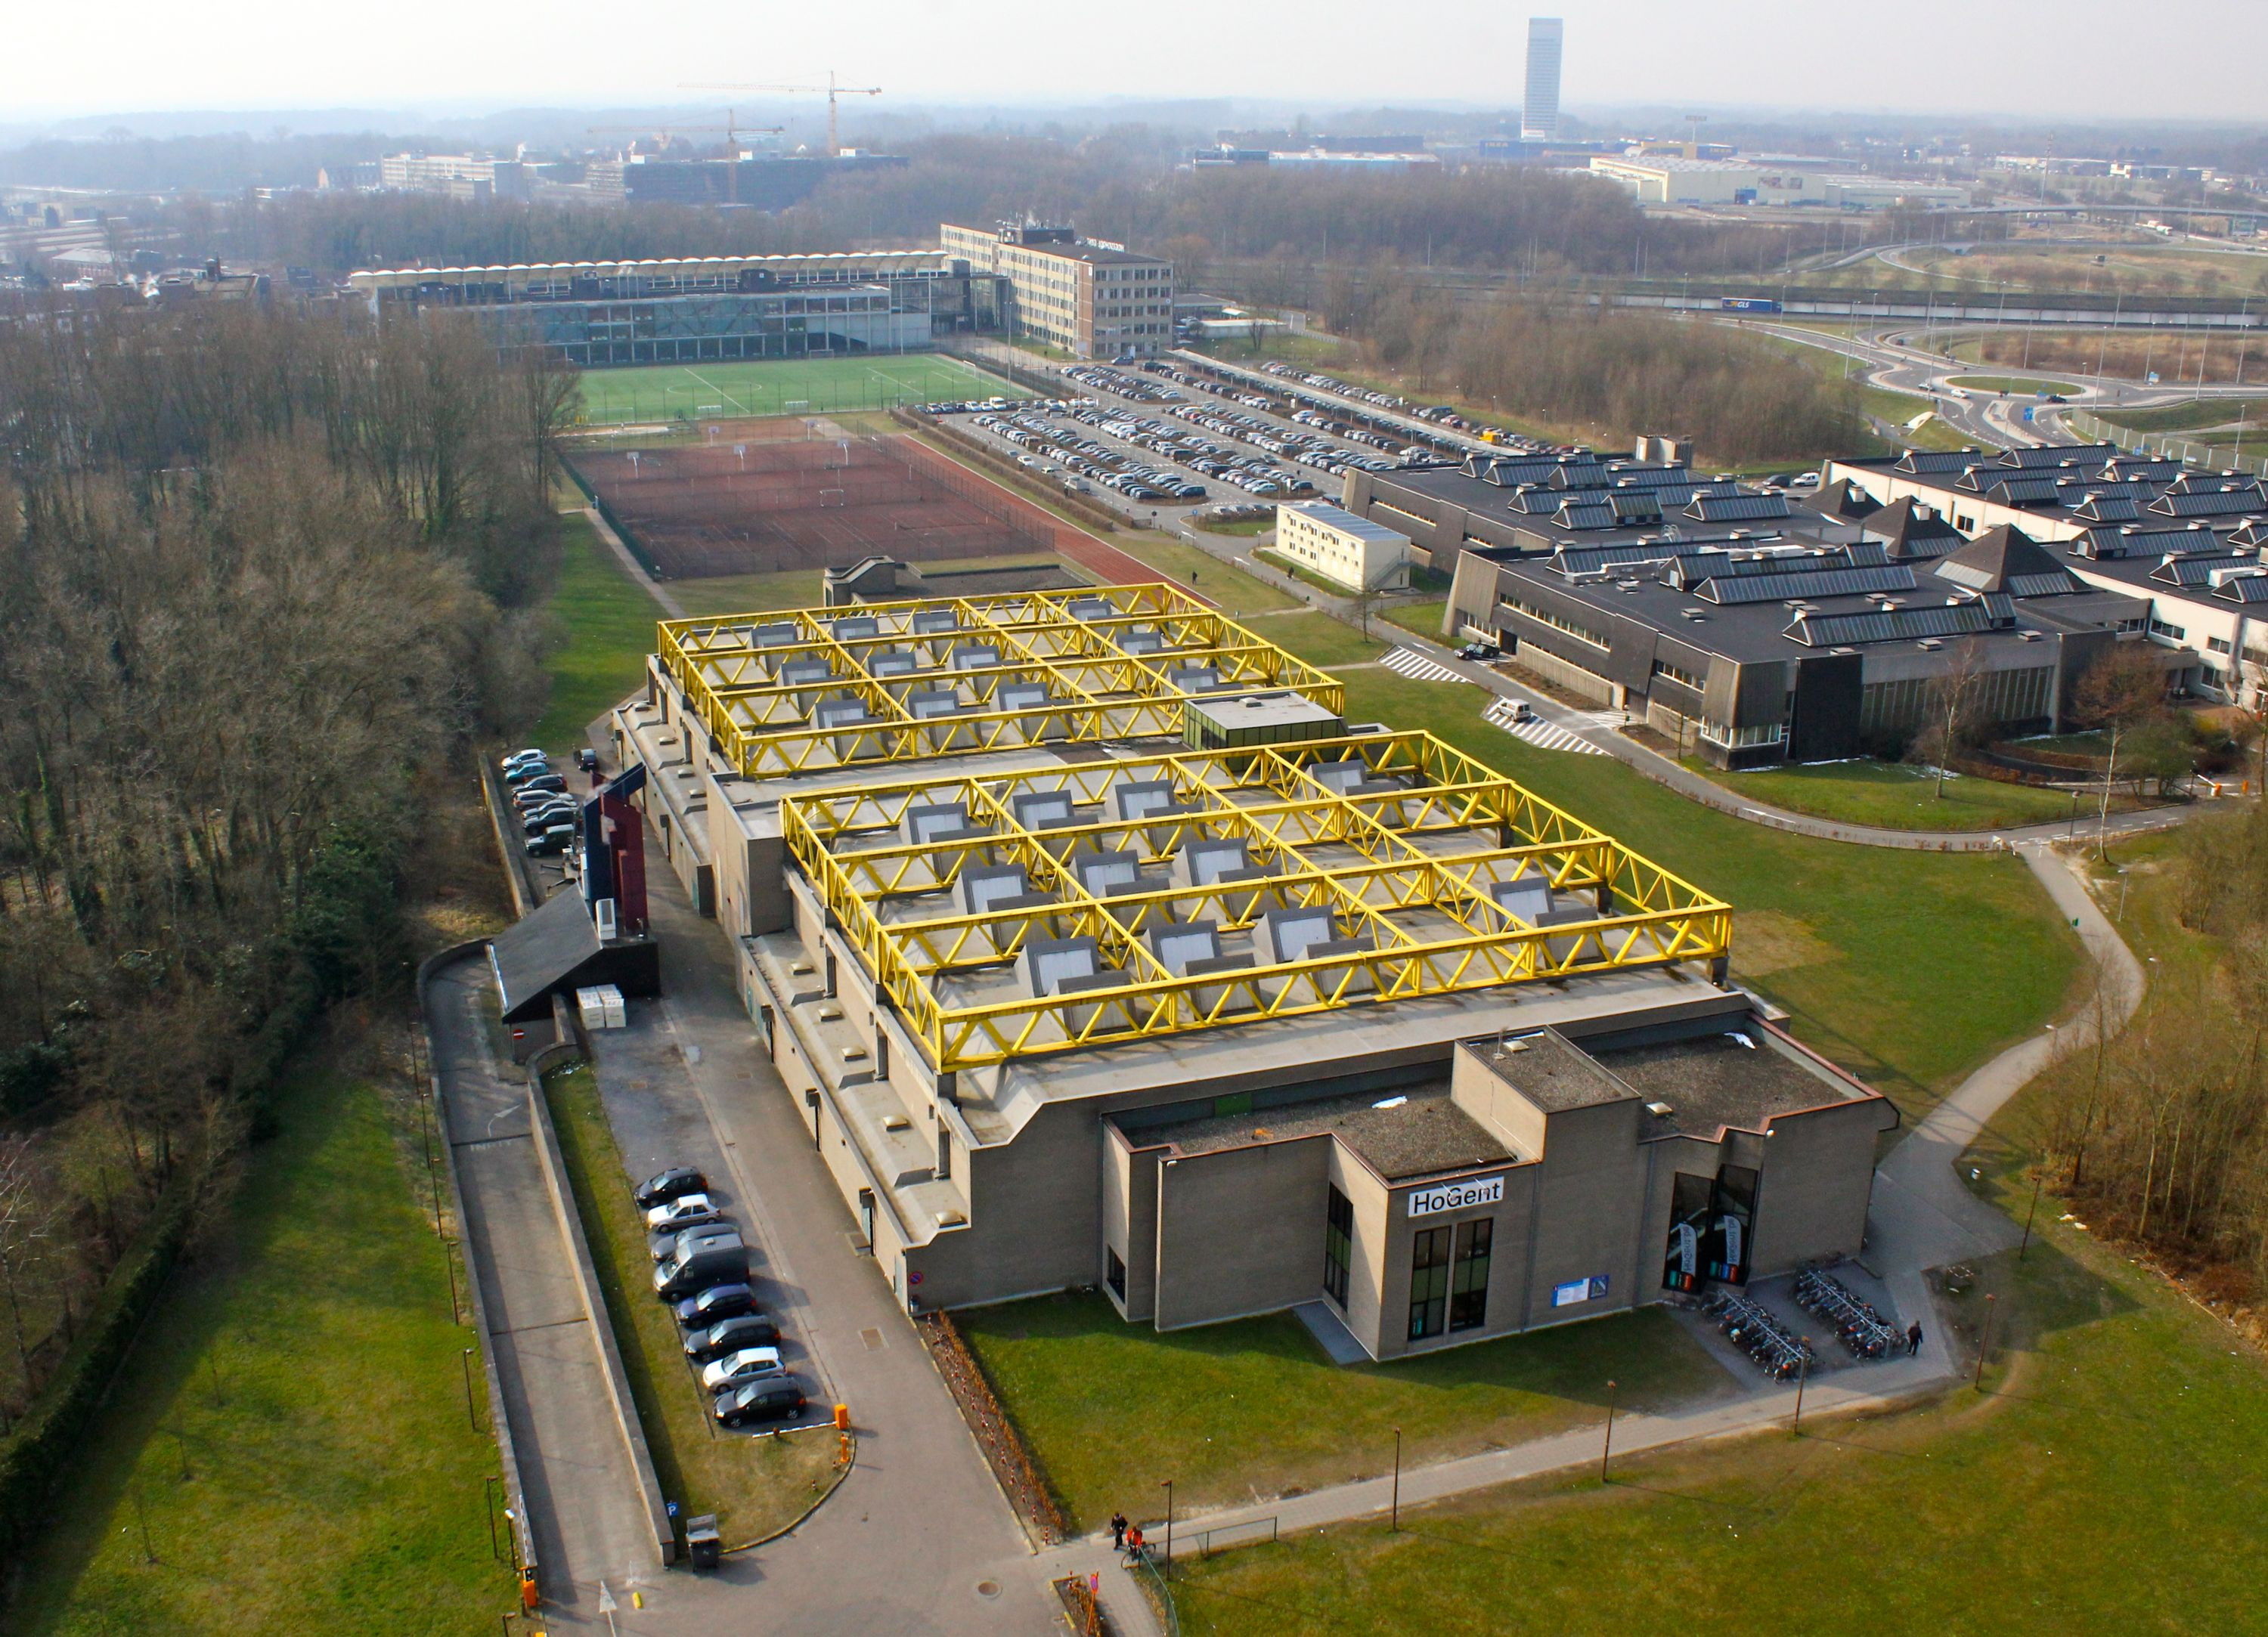
\includegraphics[width=\textwidth]
	{img/campus_hogent.JPG}
	\caption{Campus Schoonmeersen van HoGent (afbeelding gehaald van website www.hogent.be/over-hogent/campussen)}
	\label{fig:campushogent}
\end{figure}

Via \textcite{Onderwijs.vlaanderen.be2017} is het mogelijk om voor elke studierichting van de Hogeschool Gent de scores van de studenten te zien. Deze cijfers dateren van het studiejaar 2015-2016. 

Voor de richting Toegepaste Informatica (zie figuur \ref{fig:vlaanderenti}) vindt men terug dat:
\begin{itemize}
	\item 93 procent van de studenten van het mannelijk geslacht zijn.
	\item 1053 studenten deze opleiding volgden in academiejaar 2015-2016.
	\item 133 studenten behaalden dat academiejaar hun diploma, terwijl er 175 nieuwe generatiestudenten bijkwamen.
	\item slechts 44 procent van de studenten hun diploma behalen binnen 3 jaar. 25 procent behaalt het diploma pas zelfs na 5 jaar of meer.
\end{itemize}

Men ziet duidelijk bij deze richting dat vele studenten bezig zijn met deze opleiding, maar vakken moeten opnemen uit verschillende modeljaren en niet meer behoren tot een bepaald generatiejaar. Nog niet de helft van de studenten is afgestudeerd binnen de 3 voorziene jaren voor deze opleiding.

\begin{figure}
	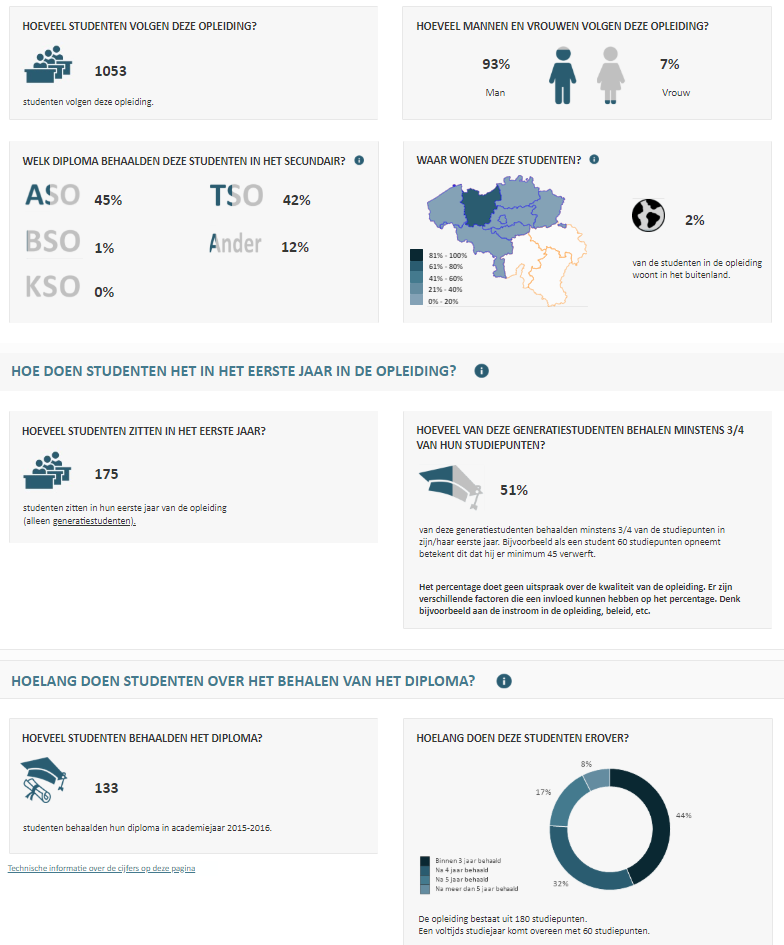
\includegraphics[width=\textwidth]
	{img/vlaanderen_ti.png}
	\caption{Statistieken studenten Hogeschool Gent Toegepaste Informatica 2015-2016
	\autocite{Onderwijs.vlaanderen.be2017}}
	\label{fig:vlaanderenti}
\end{figure}

Voor de richting Bedrijfsmanagement (figuur \ref{fig:vlaanderenbm}) ziet men dat:
\begin{itemize}
	\item maar 56 procent van deze studenten mannen zijn, de proportie vrouwen is hier veel groter hoewel dezelfde faculteit.
	\item 2257 studenten deze opleiding volgden in academiejaar 2015-2016.
	\item het aantal studenten dat begint en het aantal studenten dat afstudeert bijna exact hetzelfde zijn.
	\item 58 procent van de studenten hun diploma behalen binnen 3 jaar. 25 procent behaalt het diploma pas zelfs na 5 jaar of meer.
\end{itemize}

De richting Bedrijfsmanagement kent minder moeilijkheden met studenten die blijven studeren. Bijna 60 procent van de studenten kan in zijn modeltraject blijven.

\begin{figure}
	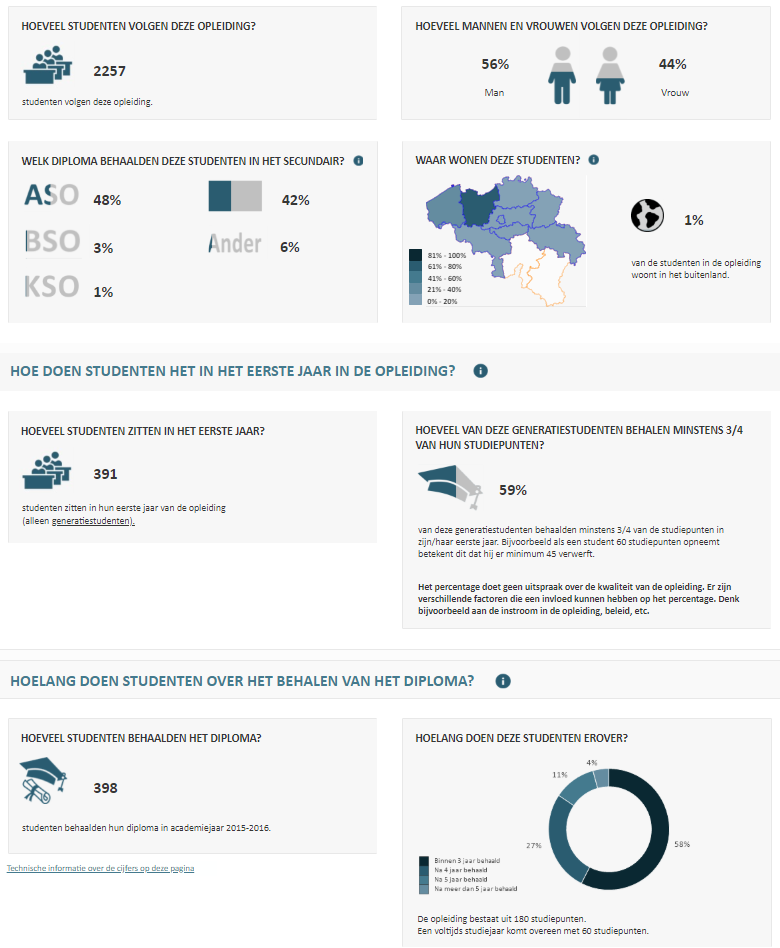
\includegraphics[width=\textwidth]
	{img/vlaanderen_bm.png}
	\caption{Statistieken studenten Hogeschool Gent Bedrijfsmanagement 2015-2016
		\autocite{Onderwijs.vlaanderen.be2017}}
	\label{fig:vlaanderenbm}
\end{figure}

Vervolgens gaan we kijken bij de faculteit Mens en Welzijn. Voor de richting Sociaal Werk (figuur \ref{fig:vlaanderensw}) kan men opmerken dat:
\begin{itemize}
	\item 71 procent van de studenten vrouwen zijn.
	\item 859 studenten deze opleiding volgden in academiejaar 2015-2016, maar dat het aantal nieuwe studenten in een dalende trend zit.
	\item 66 procent van de studenten hun diploma behalen binnen 3 jaar. 25 procent behaalt het diploma pas zelfs na 5 jaar of meer.
\end{itemize}

De richting Sociaal Werk is op papier de studierichting waarbij studenten het snelst hun diploma kunnen behalen. Het is ook een richting met het kleinste aantal studenten van de vier onderzochte richtingen in België. Opvallend is hier vooral dat deze richting in België in een negatieve trend zit.

\begin{figure}
	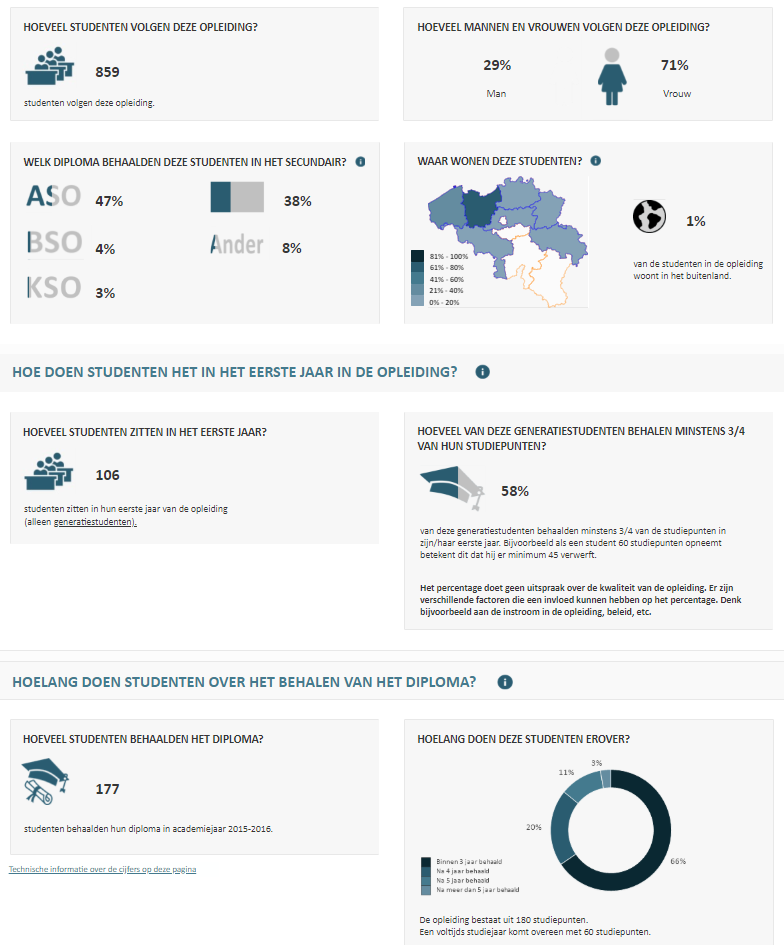
\includegraphics[width=\textwidth]
	{img/vlaanderen_sw.png}
	\caption{Statistieken studenten Hogeschool Gent Sociaal Werk 2015-2016
		\autocite{Onderwijs.vlaanderen.be2017}}
	\label{fig:vlaanderensw}
\end{figure}

Als laatste kijken we naar de richting Orthopedagogie (figuur \ref{fig:vlaanderenor}) en ziet men dat:
\begin{itemize}
	\item wel 83 procent van de studenten van het vrouwelijk geslacht zijn.
	\item 1426 studenten deze opleiding volgden in academiejaar 2015-2016
	\item 65 procent van de studenten hun diploma behalen binnen 3 jaar. Dit cijfer is bijna hetzelfde als dat van Sociaal Werk.
\end{itemize}

De richting Orthopedagogie is overduidelijk een meisjesrichting. Bijna 70 procent van de studenten behaald meer dan 3/4 van hun studiepunten die ze opnemen in het eerste jaar. Ook opvallend is dat 94 procent van de studenten hun diploma behalen binnen 4 jaar.

\begin{figure}
	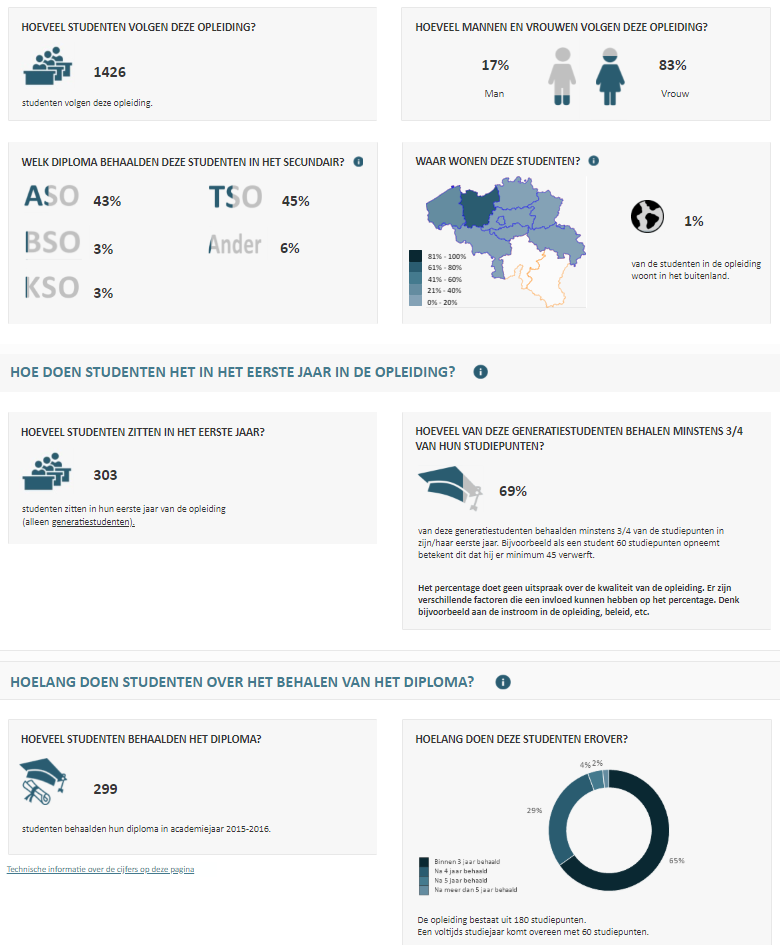
\includegraphics[width=\textwidth]
	{img/vlaanderen_or.png}
	\caption{Statistieken studenten Hogeschool Gent Orthopedagogie 2015-2016
		\autocite{Onderwijs.vlaanderen.be2017}}
	\label{fig:vlaanderenor}
\end{figure}


Als laatste eindigt men met enkele interessante tabellen, verkregen via Denis Amelynck, BI- en dataspecialist van de Hogeschool Gent. 

In figuur \ref{hogentclicks} vindt je het gedrag terug van de studenten uit de 4 Vlaamse richtingen op de leersite Chamilo, die bedoeld is voor interne uitwisseling van documenten of planningen tussen studenten en leerkrachten.


\begin{table}[]
	\centering
	\caption{Aantal clicks op Chamilo-site HoGent (Denis Amelynck, HoGent)}
	\label{hogentclicks}
	\resizebox{\textwidth}{!}{%
		\begin{tabular}{llll}
			& \textbf{2016-17} & \textbf{2017-18} & \textbf{Eindtotaal} \\
			\textbf{Bachelor in de orthopedagogie}                 & 1723679          & 1221448          & 2945127                   \\
			\textbf{Bachelor in de toegepaste informatica}         & 2383143          & 2130306          & 4513449                   \\
			\textbf{Bachelor in de toegepaste informatica - Aalst} & 444644           & 460198           & 904842                    \\
			\textbf{Bachelor in het bedrijfsmanagement}            & 3939453          & 3444629          & 7384082                   \\
			\textbf{Bachelor in het bedrijfsmanagement  - Aalst}   & 377350           & 289036           & 666386                    \\
			\textbf{Bachelor in het sociaal werk}                  & 998042           & 1132952          & 2130994                   \\
			\textbf{Eindtotaal}                             & 9866311          & 8678569          & 18544880                 
		\end{tabular}%
	}
\end{table}

Deze tabel toont duidelijk aan dat de sociale richtingen Sociaal Werk en Orthopedagogie minder tijd spenderen op de site met al het lesmateriaal. Bedrijfsmanagement is de richting waar het meest activiteit plaatsvindt, met wel meer dan 8 miljoen clicks over 2 academiejaren heen. Of dit aantoont dat bepaalde richtingen meer of minder tijd spenderen aan schooltaken of meer of minder studeren via het portaal Chamilo is een totaal andere vraag. Het geeft een beeld dat technische richtingen meer gebruik maken van het portaal dan sociale richtingen. Het is totaal fout om hieruit af te leiden welke richting het meest studeert, het meest verslaafd is aan het internet of het meest actief bezig is met school. Alles hangt natuurlijk af van de student zijn ingesteldheid, maar ook van het aantal taken of documenten dat leerkrachten uit deze studierichtingen online plaatsen.

In figuur \ref{rendementalle} ziet men het studierendement van alle studenten die participeren aan de onderzoeksrichtingen, waar in figuur \ref{rendementeerstejaar} men dit kan zien voor enkel de eerstejaarsstudenten.

\begin{table}[]
	\centering
	\caption{Studierendement van alle studenten per academiejaar (Denis Amelynck, HoGent)}
	\label{rendementalle}
	\resizebox{\textwidth}{!}{%
		\begin{tabular}{llllllll}
			& \textbf{2010-11} & \textbf{2011-12} & \textbf{2012-13} & \textbf{2013-14} & \textbf{2014-15} & \textbf{2015-16} & \textbf{2016-17} \\
			\textbf{Bachelor in de orthopedagogie}                 & 80,82\%          & 81,74\%          & 82,15\%          & 81,21\%          & 83,79\%          & 85,73\%          & 83,57\%          \\
			\textbf{Bachelor in de toegepaste informatica}         & 72,64\%          & 70,85\%          & 73,17\%          & 71,55\%          & 74,41\%          & 75,21\%          & 73,29\%          \\
			\textbf{Bachelor in de toegepaste informatica - Aalst} & 78,24\%          & 78,31\%          & 68,47\%          & 65,90\%          & 69,98\%          & 70,87\%          & 75,26\%          \\
			\textbf{Bachelor in het bedrijfsmanagement}            & 77,94\%          & 80,66\%          & 80,43\%          & 81,64\%          & 81,22\%          & 79,12\%          & 81,71\%          \\
			\textbf{Bachelor in het bedrijfsmanagement  - Aalst}   & 81,26\%          & 85,97\%          & 83,73\%          & 77,71\%          & 79,05\%          & 83,35\%          & 83,95\%          \\
			\textbf{Bachelor in het sociaal werk}                  & 76,54\%          & 78,09\%          & 80,59\%          & 81,04\%          & 77,81\%          & 80,85\%          & 80,68\%          \\
			\textbf{Eindtotaal}                                    & 78,06\%          & 79,82\%          & 79,98\%          & 79,49\%          & 80,37\%          & 80,91\%          & 80,92\%         
		\end{tabular}%
	}
\end{table}

\begin{table}[]
	\centering
	\caption{Studerendement van eerstejaarsstudenten per academiejaar (Denis Amelynck, HoGent)}
	\label{rendementeerstejaar}
	\resizebox{\textwidth}{!}{%
		\begin{tabular}{llllllll}
			& \textbf{2010-11} & \textbf{2011-12} & \textbf{2012-13} & \textbf{2013-14} & \textbf{2014-15} & \textbf{2015-16} & \textbf{2016-17} \\
			\textbf{Bachelor in de orthopedagogie}                 & 68,50\%          & 70,75\%          & 70,75\%          & 69,44\%          & 74,36\%          & 77,92\%          & 74,34\%          \\
			\textbf{Bachelor in de toegepaste informatica}         & 62,53\%          & 60,48\%          & 64,62\%          & 59,58\%          & 60,75\%          & 65,05\%          & 61,36\%          \\
			\textbf{Bachelor in de toegepaste informatica - Aalst} & 63,09\%          & 68,56\%          & 55,84\%          & 54,59\%          & 55,98\%          & 60,15\%          & 65,89\%          \\
			\textbf{Bachelor in het bedrijfsmanagement}            & 63,92\%          & 65,21\%          & 67,15\%          & 71,50\%          & 70,30\%          & 68,79\%          & 71,58\%          \\
			\textbf{Bachelor in het bedrijfsmanagement  - Aalst}   & 64,67\%          & 77,30\%          & 66,28\%          & 62,60\%          & 70,04\%          & 72,26\%          & 71,06\%          \\
			\textbf{Bachelor in het sociaal werk}                  & 66,95\%          & 65,10\%          & 67,25\%          & 70,10\%          & 67,82\%          & 70,97\%          & 67,28\%          \\
			\textbf{Eindtotaal}                                    & 65,32\%          & 67,15\%          & 67,31\%          & 67,64\%          & 69,61\%          & 71,01\%          & 70,02\%         
		\end{tabular}%
	}
\end{table}

In de afgelopen 5 jaar is in beide tabellen duidelijk te merken dat het rendement van de student stijgt. Vooral bij eerstejaarsstudenten is de stijging van 4,70 procent in 5 jaar tijd opmerkelijk. Enkel bij de richting Toegepaste Informatica, onderricht in Gent, is weinig of geen verschil te merken in studierendement. Het valt op in beide tabellen dat Toegepaste Informatica het minst hoopgevende resultaten biedt voor de student.


\section{De Haagse Hogeschool, Den Haag, Nederland}
\label{sec:haagsehogeschool}

De Haagse Hogeschool werd opgericht 1 september 1987. Ooit gegroeid uit 15 andere hbo-instellingen, heeft het zich ontwikkeld tot een instelling die jaarlijks ongeveer 3000 studenten aflevert aan de arbeidsmarkt. Deze hogeschool is niet alleen een UNESCO-hogeschool, maar het kan ook beschreven worden als een internationaal gerichte hogeschool die al studenten van meer dan 140 verschillende nationaliteiten. De hoofdvestiging is terug te vinden in het centrum van Den Haag, en heeft daarnaast nog vestigingen in Delft en Zoetermeer \autocite{HaagseHogeschool2017}. 

\begin{figure}[!h]
	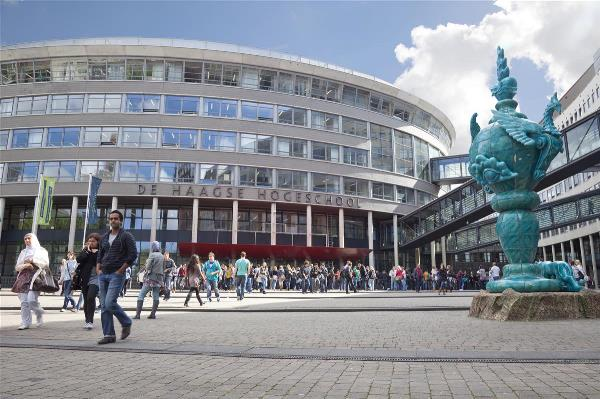
\includegraphics[width=\textwidth]
	{img/haagse_hogeschool.jpg}
	\caption{Hoofdcampus Haagse Hogeschool bij station Holland Spoor, verkregen via website www.dehaagsehogeschool.nl}
	\label{fig:haagsehogeschool}
\end{figure}

Via \textcite{Studiekeuze2017} is het mogelijk om voor elke studierichting van de Haagse Hogeschool statistieken te bekijken van het academiejaar 2016-2017. We hebben gekozen in België voor academiejaar 2015-2016 en in Nederland voor academiejaar 2016-2017, simpelweg omdat de resultaten in beide landen de meest recentste waren die ons onderzoek kon terugvinden.

Voor we deze cijfers overlopen, is het handig om te weten dat de cultuur van studeren, opvolging en toetsen compleet anders is als in België. Studenten worden door leerkrachten compleet losgelaten en horen volgens deze leerkrachten zelf complete verantwoordelijkheid te dragen over hun resultaten. Hogescholen in België hebben meestal de bedoeling om studenten hier en daar hun handje vast te houden en hen te begeleiden doorheen het traject. Nederlandse studenten merken zelf dat leerkrachten er niets om geven als je in de les op je smartphone zit. Waar in België de leerkracht de leerling een berisping zou geven of uit de klas zetten, gaan Nederlandse leerkrachten hier totaal niet op in en zien zij een student die niet gemotiveerd is en dus zijn diploma niet verdient. Waar België ook meer toelaat om vakken op te nemen door middel van volgtijdelijkheidsregels, zijn deze in Nederland strenger, waardoor studenten minder vakken kunnen opnemen door slechte examens en vervolgens de drop-out uit een richting hoger is dan in België.

Voor de richting HBO-ICT (zie figuur \ref{fig:hbo-ict} en \textcite{Studiekeuze2017}) vindt men terug dat:
\begin{itemize}
	\item 90 procent van de studenten van het mannelijk geslacht zijn.
	\item 846 studenten dez86e opleiding volgden in academiejaar 2016-2017.
	\item 315 studenten eerstejaarsstudenten zijn, waarvan 62 procent doorstroomt naar het volgende jaar.
	\item slechts 32 procent behaalt zijn diploma (van 4 modeljaren) binnen de 5 jaar.
\end{itemize}

Het is hier schokkend om te zien dat heel veel mensen elk jaar aan deze opleiding beginnen en maar 32 procent zijn diploma kan behalen binnen 5 jaar. 85 procent van de afgestudeerden dat ze deze studie opnieuw zouden kiezen en 59 procent vindt de studie een goede basis voor later. Als je dit vergelijkt met de richting in Vlaanderen, is het verschil qua doorstromen naar volgend jaren of de tijd waarin men het diploma behaalt vooral opmerkelijk.

\begin{figure}
	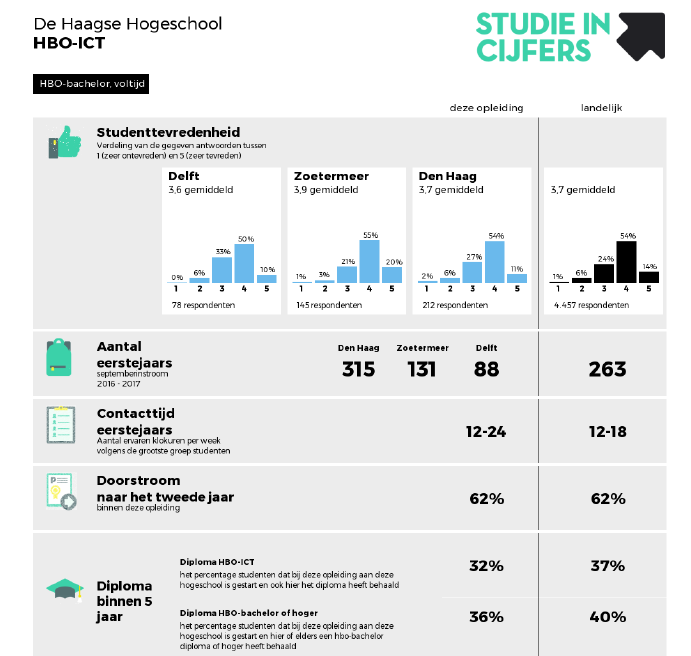
\includegraphics[width=\textwidth]
	{img/hbo-ict.png}
	\caption{Studie in cijfers HBO-ICT Haagse Hogeschool 2016-2017}
	\label{fig:hbo-ict}
\end{figure}


Voor de richting Bedrijfskunde (zie figuur \ref{fig:bedrijfskunde} en \textcite{Studiekeuze2017}) vindt men dat:
\begin{itemize}
	\item 61 procent van de studenten van het mannelijk geslacht zijn.
	\item 536 studenten deze opleiding volgden in academiejaar 2016-2017.
	\item 140 studenten eerstejaarsstudenten zijn, waarvan 58 procent doorstroomt naar het volgende jaar.
	\item slechts 21 procent behaalt zijn diploma (van 4 modeljaren) binnen de 5 jaar.
\end{itemize}

Waar het resultaat van HBO-ICT al deels schokkend was, kan hier wel gesteld worden dat het aantal dat dit diploma haalt binnen de 5 jaar bedroevend weinig is. Bedrijfsmanagement is op de Hogeschool Gent een zeer succesvolle richting, hier is het precies net andersom.

\begin{figure}
	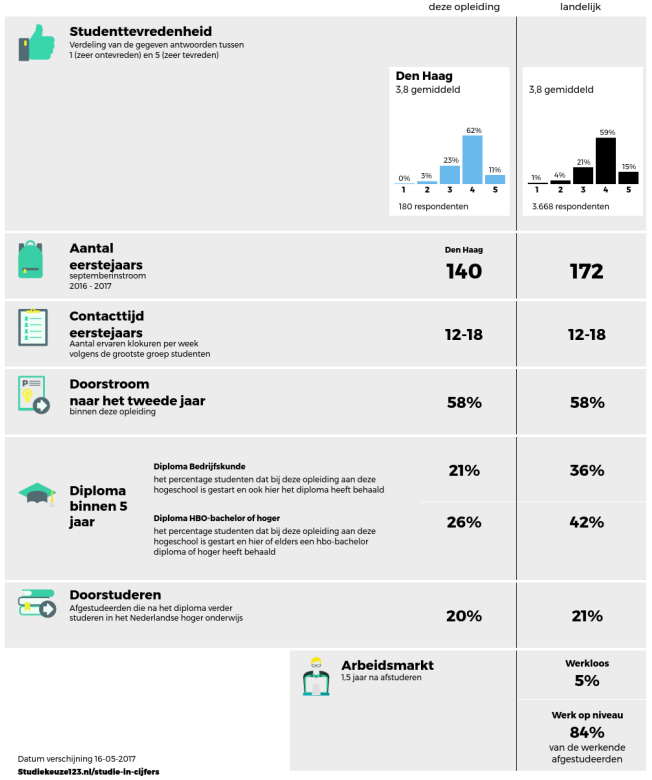
\includegraphics[width=\textwidth]
	{img/bedrijfskunde.png}
	\caption{Studie in cijfers Bedrijfskunde Haagse Hogeschool 2016-2017}
	\label{fig:bedrijfskunde}
\end{figure}

Voor de richting Social Work (zie figuur \ref{fig:socialwork} en \textcite{Studiekeuze2017}) zien we dat:
\begin{itemize}
	\item 80 procent van de studenten vrouwen zijn.
	\item 1381 studenten deze opleiding volgden in academiejaar 2016-2017.
	\item 302 studenten eerstejaarsstudenten zijn, waarvan 57 procent doorstroomt naar het volgende jaar.
	\item 37 procent behaalt zijn diploma (van 4 modeljaren) binnen de 5 jaar.
\end{itemize}

Social Work is een richting aan de Haagse Hogeschool die zeer populair is en ook redelijk goed scoort. 4 op 10 studenten kan zijn diploma binnen een redelijke termijn behalen. 

\begin{figure}
	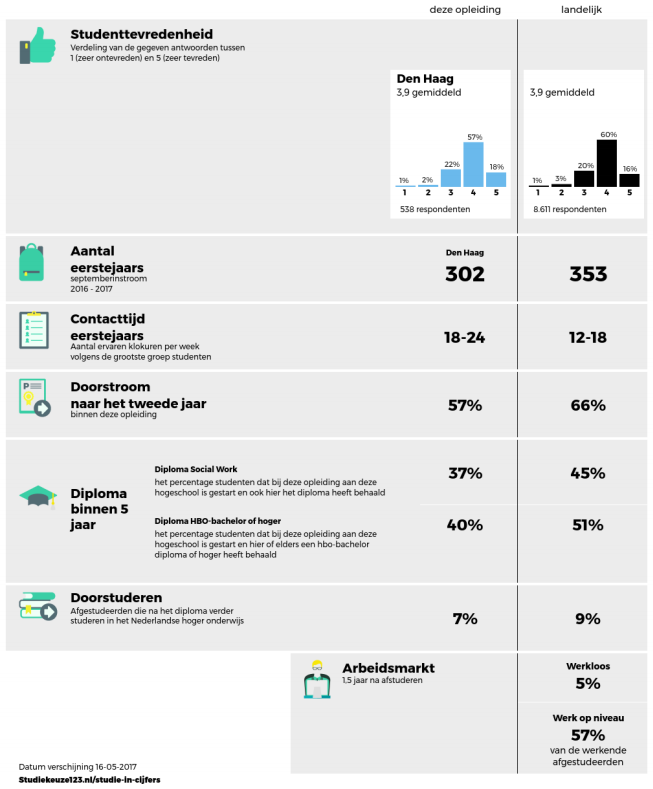
\includegraphics[width=\textwidth]
	{img/socialwork.png}
	\caption{Studie in cijfers Social Work Haagse Hogeschool 2016-2017}
	\label{fig:socialwork}
\end{figure}

Als laatse bespreken we de richting Pedagogiek (zie figuur \ref{fig:pedagogiek} en \textcite{Studiekeuze2017}) en kunnen we vaststellen dat:
\begin{itemize}
	\item 93 procent van de studenten vrouwen zijn.
	\item 444 studenten deze opleiding volgden in academiejaar 2016-2017.
	\item 159 studenten eerstejaarsstudenten zijn, waarvan 52 procent doorstroomt naar het volgende jaar.
\end{itemize}

Pedagogiek is één van de kleinere richtingen van de Haagse Hogeschool, maar scoort aanzienlijk laag als het aankomt op het aantal studenten dat doorstroomt naar het tweede jaar (landelijk gemiddelde voor deze studierichting is 70 procent). Dit houdt ofwel in dat deze richting moeilijker is in deze school dan op andere scholen in Nederland en/of dat er veel studenten afhaken tijdens het eerste jaar. 

\begin{figure}
	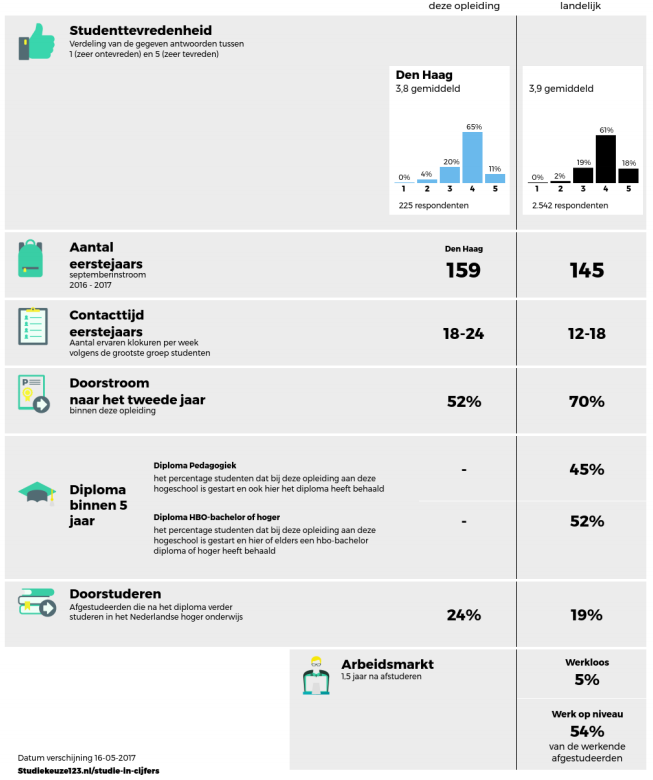
\includegraphics[width=\textwidth]
	{img/pedagogiek.png}
	\caption{Studie in cijfers Pedagogiek Haagse Hogeschool 2016-2017}
	\label{fig:pedagogiek}
\end{figure}

Nu we al deze resultaten op een rijtje zetten, kunnen we zien dat de Haagse Hogeschool het ofwel moeilijk heeft om studenten hun diploma te doen behalen, ofwel ze de opleiding te moeilijk maken en er daardoor een grote drop-out is van studenten. Men mag ook niet vergeten dat Den Haag een zeer multiculturele stad is, met veel verschillende talen en gebruiken, wat het zowel voor studenten als leerkrachten niet gemakkelijker maakt. De Haagse Hogeschool is wel een van de best scorende hogescholen van de grote steden van Nederland (5,6 op 10). In Amsterdam of Rotterdam scoren de hogescholen zelfs nog lager \autocite{AD-PeterKoop2017}.

\newpage
\section{Praktijkonderzoek Probleemoplossend Denken 1, Toegepaste Informatica, Hogeschool Gent, België}
\label{sec:pod1gent}

Voor het praktijkonderzoek is gekozen om vakken te testen uit de richting waarvoor deze bachelorproef is geschreven. Zo is het onderzoek uitgekomen bij het vak Probleemoplossend Denken 1. Dit vak wordt onderricht in het tweede semester van het eerste modeljaar van de richting Toegepaste Informatica te Gent. Eén van de lectoren voor dit vak, Mevrouw Anita Bernard, heeft de praktijktesten aan haar klassen gegeven op woensdag 9 mei. 

Dankzij Denis Amelynck, data-analyst van de Hogeschool Gent, heeft men volgende gegevens bemachtigd die aantonen hoe het is gesteld met de resultaten voor het vak Probleemoplossend Denken 1 uit de richting Toegepaste Informatica (modeljaar 1) van de Hogeschool Gent.

Het vak heeft volgens \textcite{Studiegids2017} volgende doelstellingen voor studenten:
\begin{itemize}
	\item De principes van algoritmische analyse verwerven
	\item Vraagstukken in programmeerbare methoden kunnen omzetten6
	\item Inzicht verwerven in de verschillende datastructuren.
\end{itemize}

In het academiejaar 2016-2017 was het examencijfer voor POD1 gemiddeld 10,82 op 20, wat aantoont dat het vak door studenten wordt beschouwd als een moeilijk examen. Het examen is gesloten boek, waarbij de cursus in het begin van het semester beschikbaar wordt gesteld voor de studenten via Chamilo. Tijdens dat academiejaar waren 219 studenten ingeschreven in Gent om deel te nemen aan het examen. 48 studenten ofwel 21,92 procent van de studenten was afwezig voor het examen en 98 van de 171 studenten die aanwezig waren ofwel 57,31 procent van de aanwezige studenten scoorden een cijfer lager dan 10 op 20 (Denis Amelynck, HoGent).

In figuur \ref{pod1ex} ziet u de distributie van de gegeven punten voor dit vak in het academiejaar 2016-2017.

\begin{landscape}
	\begin{table}[]
		\centering
		\resizebox{\textwidth}{!}{%
			\begin{tabular}{@{}llllllllllllllllllllll@{}}
				\toprule
				& 0 & 1  & 2  & 3  & 4  & 5  & 6  & 7  & 8  & 9  & 10 & 11 & 12 & 13 & 14 & 15 & 16 & 17 & 18 & AFW & Eindtotaal \\ \midrule
				Probleemoplossend denken I  (TI)         & 3 & 9  & 12 & 15 & 23 & 11 & 18 & 22 & 15 & 14 & 39 & 14 & 12 & 16 & 8  & 10 & 4  & 4  & 2  & 80  & 331        \\
				Probleemoplossend denken I  (TI) (Aalst) &   & 1  & 3  & 8  & 6  & 9  & 8  & 4  & 3  & 2  & 7  & 5  & 5  & 4  & 5  & 4  & 2  & 3  & 3  & 11  & 93         \\
				Eindtotaal                               & 3 & 10 & 15 & 23 & 29 & 20 & 26 & 26 & 18 & 16 & 46 & 19 & 17 & 20 & 13 & 14 & 6  & 7  & 5  & 91  & 424        \\ \bottomrule
			\end{tabular}%
		}
		\caption{distributie examenresultaten Probleemoplossend Denken 1 academiejaar 2016-2017}
		\label{pod1ex}
	\end{table}
\end{landscape}

\section{Vragen voor Onderzoek}
\label{sec:eindliteratuur}

Uit deze studie en alle bovenstaande informatie halen we volgende onderzoeksvragen, die hopelijk beantwoord zullen worden door de resultaten in volgende hoofdstukken:

\begin{itemize}
	\item Heeft het gebruik van smartphones en laptops tijdens de lessen mogelijks een invloed op de slaagcijfers en kennis van de student? (Hoofdvraag)
	\item Heeft geslacht, relatiestatus of leeftijd van de student een invloed op de aantrekkingskracht die deze devices hebben op de student?
	\item Is er een verschil in omgang met devices tussen Nederlandse en Vlaamse studenten?
	\item Wat denken studenten zelf over de invloed van smartphones op hun resultaten?
	\item Is er een verschil in gebruik van smartphones en in resultaten tussen studenten uit een sociale richting en studenten uit een richting die IT-gerelateerd is?
	\item Is er een direct positief effect op de student in het klaslokaal wanneer de smartphone en laptop volledig uit beeld verdwijnen?
\end{itemize}
